
\subsection{OpenStack ongoing extensions}
\label{subsec:ga_extensions}
\subsubsection{Trio2o} 
Tiro2o attempts to achieve scalability of an OpenStack deployment by introducing the idea of API gateways. The core concepts of Trio2o are (1) an OpenStack deployment is divided into several sites where each site runs all key OpenStack services (2) Trio2o exposes a single OpenStack API endpoint to end-users giving them a view of a large (single) cloud with several availability zones that that represent the several sites  (3) Trio2o uses standard OpenStack APIs to communicate to the various OpenStack sites (see Figure \ref{fig:Trio2oArch}). In the original design \cite{https://wiki.openstack.org/wiki/OpenStack_cascading_solution}, Trio2o was realized by a standard OpenStack instance that uses custom drivers for each service (e.g., a nova plugin in the top instance is capable managing the bottom instances through the nova-api interface). In the current design, API gateways for the specific services expose the single interface while forwarding the request to the appropriate bottom site.  

\begin{figure}[htbp]
\begin{center}
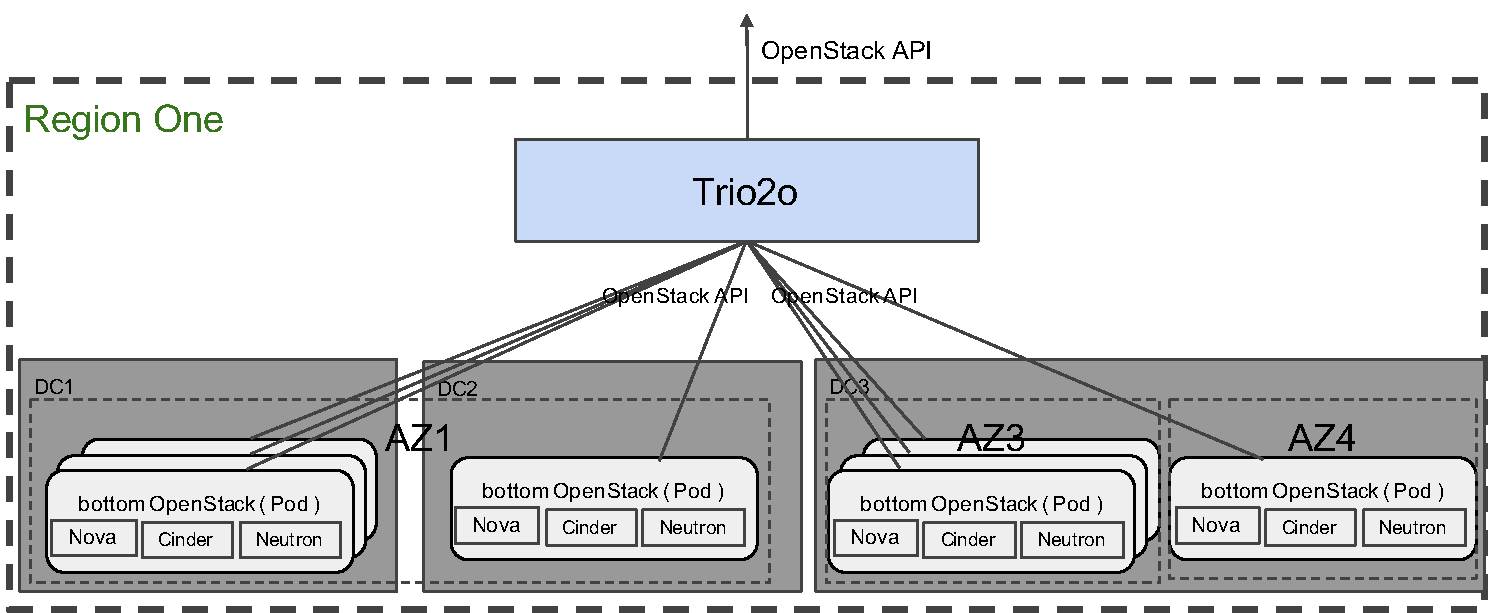
\includegraphics[width=0.5\textwidth]{trio2oarch}
\caption{High-level architecture of Trio2o (https://docs.google.com/presentation/d/16laTyn4ra-446v4p0kwMnpgHqwzMsz1r6QeiSI2Kq2M/edit?usp=sharing)}
\label{fig:Trio2oArch}
\end{center}
\end{figure}

In its current implementation, Trio2o assumes a site is an OpenStack region that shares Keystone and Glance services. The top level implements gateway services for OpenStack Nova and OpenStack Cinder services while networking functionality is provided via the spinoff service TriCircle. Beyond the gateway services, Trio2o also includes two other components: an admin API that allows, among others, managing bottom instances and an Xjob service that allows other components of Trio2o to execute asynchronous jobs. 

Trio2o fulfills the requirements for Level 1 and 2. For level 3, a disconnected site will continue to run its workloads but it will not be possible to start new workloads on it until the disconnection is restored. All sites with connectivity with Trio2o will continue to operate normally. Level 4.1a is not an issue as the current implementation uses a shared glance across all sites. Trio2o leverages Tricircle for 4.1b and 4.1c. 4.1d is possible due to the global glance service. 4.1e may be implemented as an Xjob job, provided that cross-region VM migration is supported natively by the bottom OpenStack instances (not currently supported). level 4.1f may be supported provided that it is supported natively by the bottom OpenStack instances (not currently supported) whie 4.1f is not supported. Levels 4.2  and 5 are mostly not yet supported in the current implementation, but there is nothing in the architecture that prevents this from it being realized. Level 6.a will not be an issue as long as the API version numbers are synchronized, but even with bottom sites with services having different API versions, there is nothing in the design that prevents that from implementing such a support. Level 6.b and 7 will be a challenge to implement due to the services that need to be shared across the several sites.  
\subsubsection{TriCircle}
\subsubsection{Kingbird}
\subsubsection{oaktree}

